%%%%%%%%%%%%%%%%%%%%%%%%%%%%%%%%%%%%%%%%%
% XXV Simposio Chileno de Física, LaTeX Template, Versión 1 (8 may 2026)
% vmunoz@fisica.ciencias.uchile.cl
% Basado en versión previa de 
% fabian.torres@ufrontera.cl    (7 Junio 2024)
% daniel.salinas@sansano.usm.cl (12 Septiembre 2022)
%%%%%%%%%%%%%%%%%%%%%%%%%%%%%%%%%%%%%%%%%
% Método de compilación:  
%				
%				LaTeX->PDF
%
%%%%%%%%%%%%%%%%%%%%%%%%%%%%%%%%%%%%%%%%%
%
%                                                    INSTRUCCIONES SOBRE EL DOCUMENTO
%
% - Subrayar al expositor del trabajo,
% -	Borrar el texto en rojo y este comentario
% -	No se debe modificar los tamaños de letra.
% -	El título del trabajo no debe superar 2 líneas, o 30 palabras o 140 caracteres incluyendo espacios.
% -	Preferentemente, incluya sólo el correo electrónico del expositor del trabajo.
% -	Incluya un máximo de 5 autores. En caso de tener más de 5 autores, seleccione los principales incluyendo al expositor, y agregue et al %   al listado para incluir al resto.
%
%-----------------------------------------

%----------------------------------------------------------------------------------------
%	CONFIGURACIÓN DEL DOCUMENTO
%----------------------------------------------------------------------------------------

\documentclass[11pt,spanish]{article}

\usepackage[spanish]{babel}
\usepackage{epsfig,graphicx}
\usepackage{amsmath, amsthm, amsfonts}
\usepackage[hmarginratio=6:5,top=32mm,columnsep=11mm,textwidth=178mm]{geometry}
\usepackage[makeroom]{cancel} %FT - para incluir simplificaciones en ecuaciones
\usepackage{multicol} %FT - para generar varias columnas en una seccion del documento
\usepackage[hang,small,labelfont=bf,up,textfont=it,up]{caption} % Custom captions under/above floats in tables or figures
\usepackage{subcaption} % Paquete esencial
\usepackage{booktabs} % Horizontal rules in tables
\usepackage{float} % Required for tables and figures in the multi-column environment - they need to be placed in specific locations with the [H] (e.g. \begin{table}[H])
\usepackage{hyperref} % For hyperlinks in the PDF
\usepackage{paralist} % Used for the compact item environment which makes bullet points with less space between them
\usepackage[version=4]{mhchem}
\usepackage{amsmath}
\addcontentsline{toc}{section}{Title of the section}
\usepackage{titlesec} % Allows customization of titles
\usepackage{fancyhdr} % Headers and footers

\newcommand\blfootnote[1]{%
  \begingroup
  \renewcommand\thefootnote{}\footnote{#1}%
  \addtocounter{footnote}{-1}%
  \endgroup
}

\pagestyle{fancy} % All pages have headers and footers
\fancyhead{} % Blank out the default header
\fancyfoot{} % Blank out the default footer
\renewcommand{\headrulewidth}{3pt}
\renewcommand{\footrulewidth}{0pt}
%-----------------------------------------------------------------------------------------
% AGREGUE AQUÍ UNA DE LAS ÁREAS DEFINIDAS EN LA PÁGINA WEB DEL SIMPOSIO www.sochifi2014.udec.cl
%-----------------------------------------------------------------------------------------


\fancyhead[L]{\small 	Óptica y \\ Física Cuántica } % Custom header text
\fancyhead[R]{{\bf XXV Simposio Chileno de Física} \\  23 al 26 de
  noviembre de 2026 \\  Santiago, Chile} % Custom header text
\fancyfoot[RO,L]{\thepage} % Custom footer text

\linespread{1} %

%----------------------------------------------------------------------------------------
%	TÍTULO Y AUTORES. SUBRAYAR AL EXPOSITOR
%----------------------------------------------------------------------------------------

\title{\vspace{-5mm}\fontsize{16pt}{10pt}\selectfont \textbf{Desarrollo de un láser de bajo costo, con ancho de línea estrecho y amplificación cónica.}} % Article title
\vspace{-3mm}
\author{
\normalsize \underline{Florencia Fuentes J$^{1*}$}, Nicolás Vera$^{1}$, Pablo Solano$^{1\dagger}$ \\
\vspace{-1mm}
\small $^1$ Universidad de Concepción, Concepción. \\
\small $*$\href{mailto:flofuentes2021@udec.cl}{flofuentes2021@udec.cl},
\quad
$\dagger$\href{mailto:psolano@udec.cl}{psolano@udec.cl}
}
\date{}
\pagestyle{empty}
%----------------------------------------------------------------------------------------
\nofiles
\newcommand{\seccion}[1]{\noindent {\Large\textbf{#1}}\\}
	
\begin{document}
\maketitle
\thispagestyle{fancy} % All pages have headers and footers
\pagenumbering{gobble}

%----------------------------------------------------------------------------------------
%	CONTENIDO
%----------------------------------------------------------------------------------------
\seccion{Resumen}
Los láseres son la base de la mayoría de los experimentos de óptica y física atómica. Para construir una trampa magneto-óptica (MOT) es esencial contar con fuentes de luz controlada, focalizada y de alta intensidad; sin embargo, estos sistemas pueden superar las decenas de miles USD, lo que los hace inaccesibles para laboratorios emergentes. Esto motiva el desarrollo de un sistema láser de bajo costo con estrecho ancho de línea y alta potencia, construido a partir de componentes comerciales, capaz de satisfacer los requisitos de experimentos de espectroscopía atómica y atrapamiento de átomos.


%Incluya ecuaciones, tablas y figuras si es necesario.
\begin{multicols}{2}
\seccion{Desarrollo}
Elaboramos un láser de diodo de cavidad externa (ECDL) controlado en corriente por un circuito Libbrecht–Hall de bajo ruido, en configuración Littrow, cuya cavidad es controlada por un piezoeléctrico que permite sintonizar y estabilizar con precisión la longitud de onda emitida. Esta configuración
es fundamental para la espectroscopía de alta resolución y para el atrapamiento de átomos alcalinos como el $\ce{^{87}_{}Rb}$ cuyo ancho de línea natural (FWHM) en la transición D2 ( $\ce{5^{2}S_{1/2}}$ $\rightarrow$ $\ce{5^{2}P_{3/2}}$) es de ~$6,07$ MHz. El ancho de línea del láser se redujo mediante retroalimentación óptica y se caracterizó con la técnica autoheterodina. El espectro se describe mediante la densidad espectral de potencia (PSD) derivada del teorema de Wiener-Khinchin. \footnote{
  
  \begin{minipage}{\textwidth}
    \begin{equation}
      %\begin{split}
      S(\omega, \tau) = \frac{\frac{1}{2} P_0^2 \tau_c}{1 + {\omega \pm \Omega}^2 \tau_c^2} \left\{ 1 - e^{-\frac{-|\tau|}{\tau_c}} [\cos(\omega \pm \Omega)] \tau \right\} 
      \\ + \frac{\sin(\omega \pm \Omega) |\tau|}{(\omega \pm \Omega) \tau_c} + \frac{1}{2} P_0^2 \pi e^{-\frac{-|\tau|}{\tau_c}} \delta(\omega \pm \Omega).
      %\end{split}
    \end{equation}Donde, $\tau_c$ es el tiempo de coherencia, $\Omega$ es el desplazamiento de frecuencia de un modulador acusto óptico (AOM) y $P_0$ es la potencia del láser.
  \end{minipage}
  }

  Observamos que sin retroalimentación óptica, el FWHM medido es de ~4,76 MHz versus con retroalimentación que se reduce a ~24,8 kHz, valor inferior al ancho de línea natural del $\ce{^{87}_{}Rb}$. Sin embargo los ECDL producen potencias inferiores a 100 mW. Implementamos una configuración MOPA (Master Oscillator Power Amplifier) que utiliza un amplificador cónico (TA) para incrementar la potencia óptica conservando ancho de línea del láser.
%\columnbreak
\begin{minipage}{0.7\textwidth}
  \begin{figure}[H]
      \begin{subfigure}{0.35\textwidth}
          \begin{flushleft}
           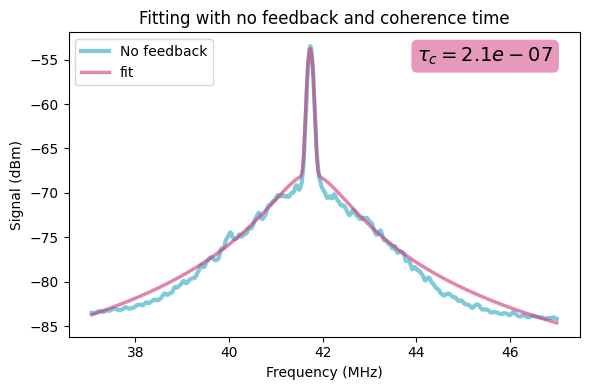
\includegraphics[width=\textwidth]{nofeed.png} 
           %\subcaption{PSD medida sin retroalimentación.}
          \end{flushleft}    
      \end{subfigure} \hspace{0.005\textwidth}
      \begin{subfigure}{0.35\textwidth}
          \begin{flushright}
            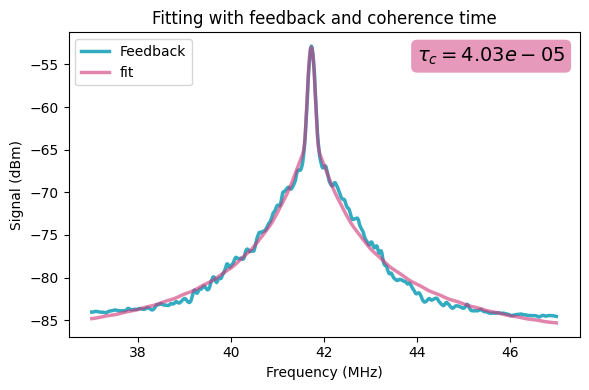
\includegraphics[width=\textwidth]{feed.png}
            %\subcaption{PSD medida con retroalimentación.}
          \end{flushright}
      \end{subfigure}
  \end{figure} 
\end{minipage}
  Logramos implementar un sistema láser de bajo costo con estrecho ancho de línea y alta potencia, apto para experimentos de espectroscopía atómica y atrapamiento de átomos. Este desarrollo demuestra que la física de frontera es accesible en entornos con recursos económicos restringidos.
  \noindent {\large\textbf{Referencias}} 
  
  \noindent[1] L.cE. Richter, et al. \href{https://doi.org/10.1109/JQE.1986.1072909}{10.1109/JQE.1986.1072909}.
  \noindent[2] C. J. Hawthorn, et al. doi: \href{https://doi.org/10.1063/1.1419217}{10.1063/1.1419217}.
  \noindent[3] M. Chi, et al. doi: \href{https://doi.org/10.1364/OPEX.13.010589}{10.1364/OPEX.13.010589}.
  \noindent[4] C.M. Seck, et al. doi: \href{https://doi.org/10.1063/1.4953330}{10.1063/1.4953330}

\end{multicols}




% \begin{figure}[H]
% \centerline{\includegraphics[width=3cm]{sochifilogo.png}}
% \end{figure}






\end{document}
